\section{Software Overview}
\label{sw_sec}

This section presents an overview of the firmware developed for the iNEMO board and the application developed for the Android device.

\subsection{Firmware}
\label{fw_sec}

The firmware for the iNEMO board is based on the real-time operating system FreeRTOS, version 7\footnote{The FreeRTOS Project: \url{http://www.freertos.org}}. Most of the code is taken from the original code furnished by STMicroelectronics: in particular, the libraries to manage sensors, ports and internal communication have been totally reused without any change. The main contributes to the firmware of this work are the support of Android Open ADK and the implementation of a set of tasks to allow communication with the Android device.

As said in section \ref{hw_sec}, USB Host functionality is provided by an USB Host Shield that integrates the Maxim MAX3421E USB host controller. Hence, to support the communication on the USB through the MAX3421E, USB control library and MAX3421E driver, developed by Circuits@Home\footnote{Circuits@Home: \url{http://www.circuitsathome.com}} for the Arduino Platform, have been adapted to STM32 microcontrollers family. At the higher level of the software stack there is the Android Accessory library: it has been implemented according to the indications furnished by the Android Developer's Guide. {\bf Figure \ref{fig:sw_stack}} shows the software stack for the support of Android Open ADK. 

\begin{center}
	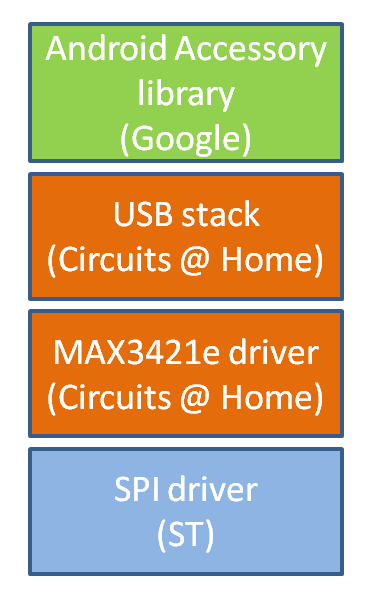
\includegraphics[width=0.5\linewidth]{pics/sw_stack.eps}
	\captionof{figure}{Software stack for the support of Android Open ADK.}
	\label{fig:sw_stack}
\end{center}

The communication with the Android device is guaranteed by 3 tasks:

\begin{itemize}
 	\item Accessory Task: it manages the communication according to the Accessory protocol and can awake the Command Task in order the process the messages received from the Android device.
	\item Command Task: it parses the messages received from the Android device and builds the response messages. It can awake the Data Task.
	\item Data Task: it sends messages containing data received from the sensors integrated on the board.
\end{itemize}  

The Accessory task is always active: it examines the USB bus to check if an Android device is attached. In case a device is found, the Accessory Task establishes a connection with it (see section \ref{adk_sec}). Once the device is in Accessory mode, the Accessory Task waits for messages from it. When a message is received, it is sent to the queue on which the Command Task is waiting for. Then, the Command Task can retrieve the message sent from the device and parse it. According to the contents of the message, the Command Task sends an appropriate response message and eventually enables or disables the Data Task. When enabled, the Data Task sends the data retrieved from the sensors of the board to the Android device.

Keil uVision 4 has been used as development environment and debugger for the realization of the firmware. The main issue encountered in using this IDE was the limitation on the code size (32KB) present in the free version (MDK-Lite): this forced us to eliminate, for the moment, the support of gyroscopes, magnetometer and pressure sensor, even if the libraries for them are ready to be used. For this reason, one of the future goal for this work is to implement a completely open compile chain (probably based on gcc), in order to get rid of the limitations imposed by Keil uVision IDE.

\subsection{Android Application}
\label{apk_sec}

The Android application is composed of 3 activities:

\begin{itemize}
	\item UsbAccessoryActivity: this activity is responsible for detecting if the board is attached to the device. In case the board is attached, after having requested the permission to the user, this activity starts the INemoDemoActivity and terminates. An intent filter for the \textit{USB\_ACCESSORY\_ATTACHED} action is added to the Manifest, in order to make the UsbAccessoryActivity capable of detecting the iNEMO board.
	\item INemoDemoActivity: this is the main activity of the application. It is responsible for managing the communication with the board and updating the layout of the application.
	\item SettingsActivity: this activity lets the user modify the acquisition parameters. In particular it is possible to modify the acquisition rate, choose the enabled sensors or change the settings of the enabled sensors.

\end{itemize}


The communication protocol presented in section \ref{cp_sec} has been fully implemented in the class CommunicationFrame. The details regarding the frame format of the messages are all contained in this class: this allows separating the specific implementation of the protocol from the rest of the application, allowing in this way to easily change the communication protocol without much effort.


When the application is started, if the iNEMO board is detached, the splash screen shown in {\bf Figure \ref{fig:no_dev}} is displayed.

\begin{center}
	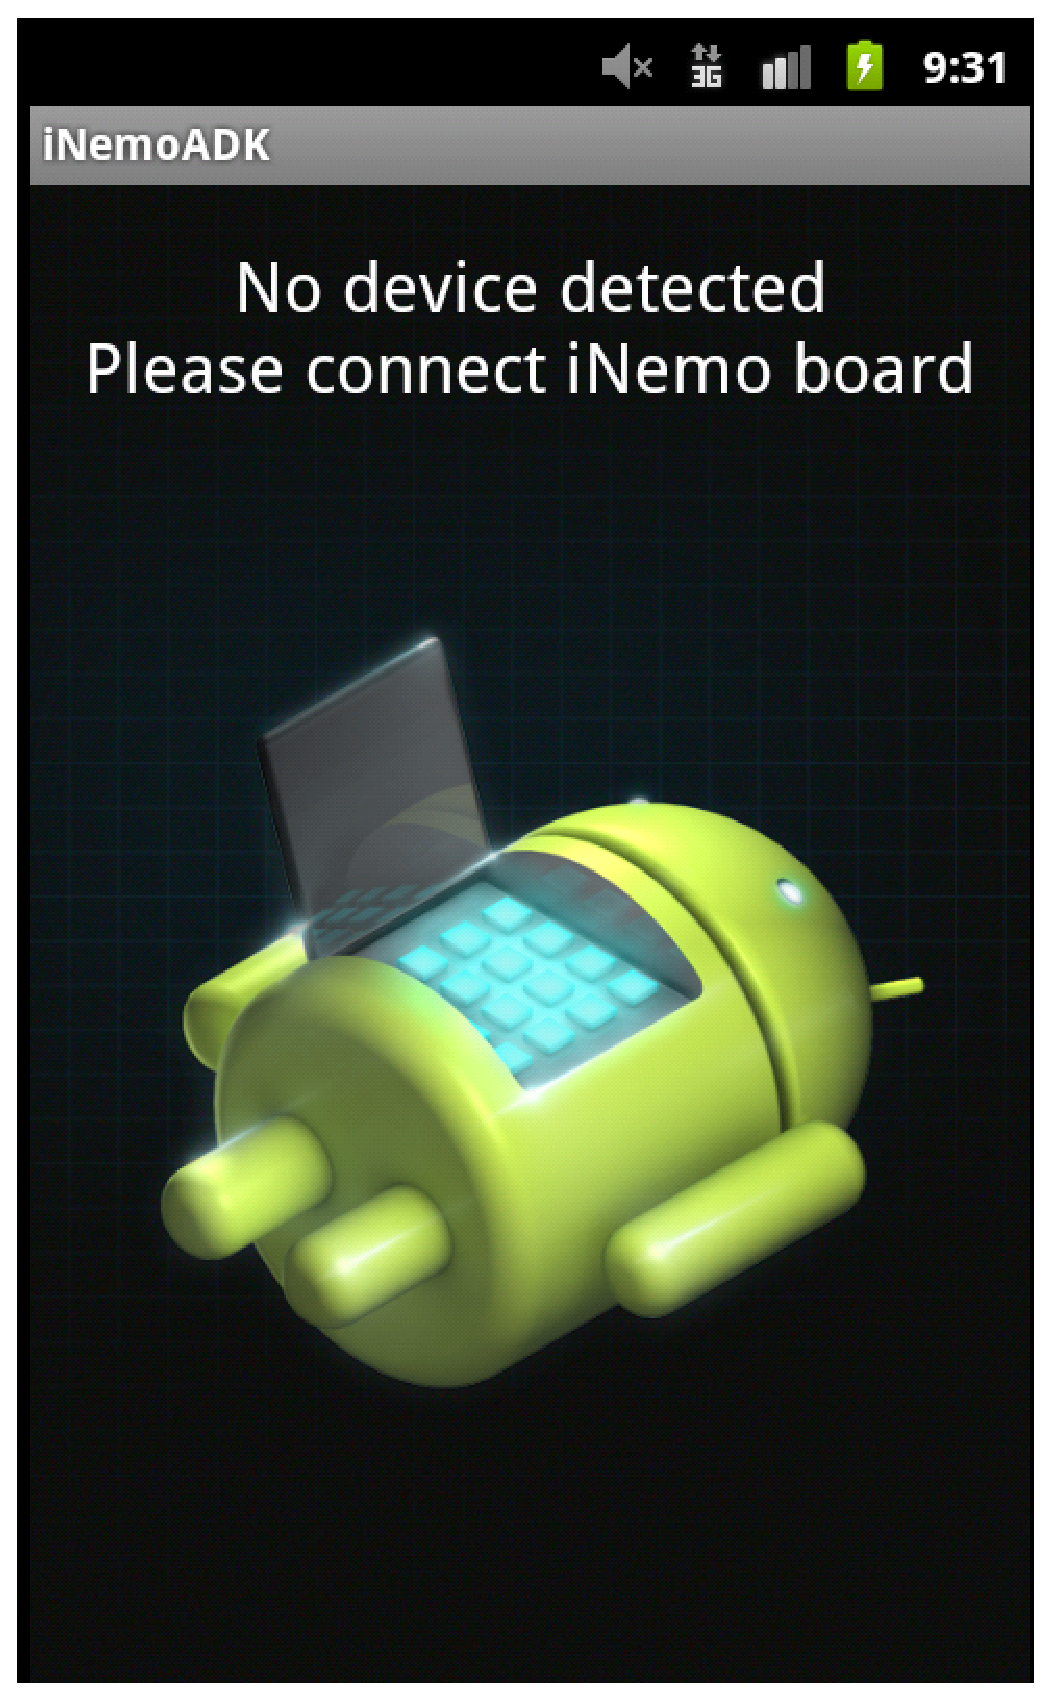
\includegraphics[width=0.6\linewidth]{pics/no_dev.eps}
	\captionof{figure}{Splash screen shown when the iNEMO board is detached.}
	\label{fig:no_dev}
\end{center}

When the board is attached, some introductive information on the board is shown and the user has the possibility to start the connection (see {\bf Figure \ref{fig:connect}}).

\begin{center}
	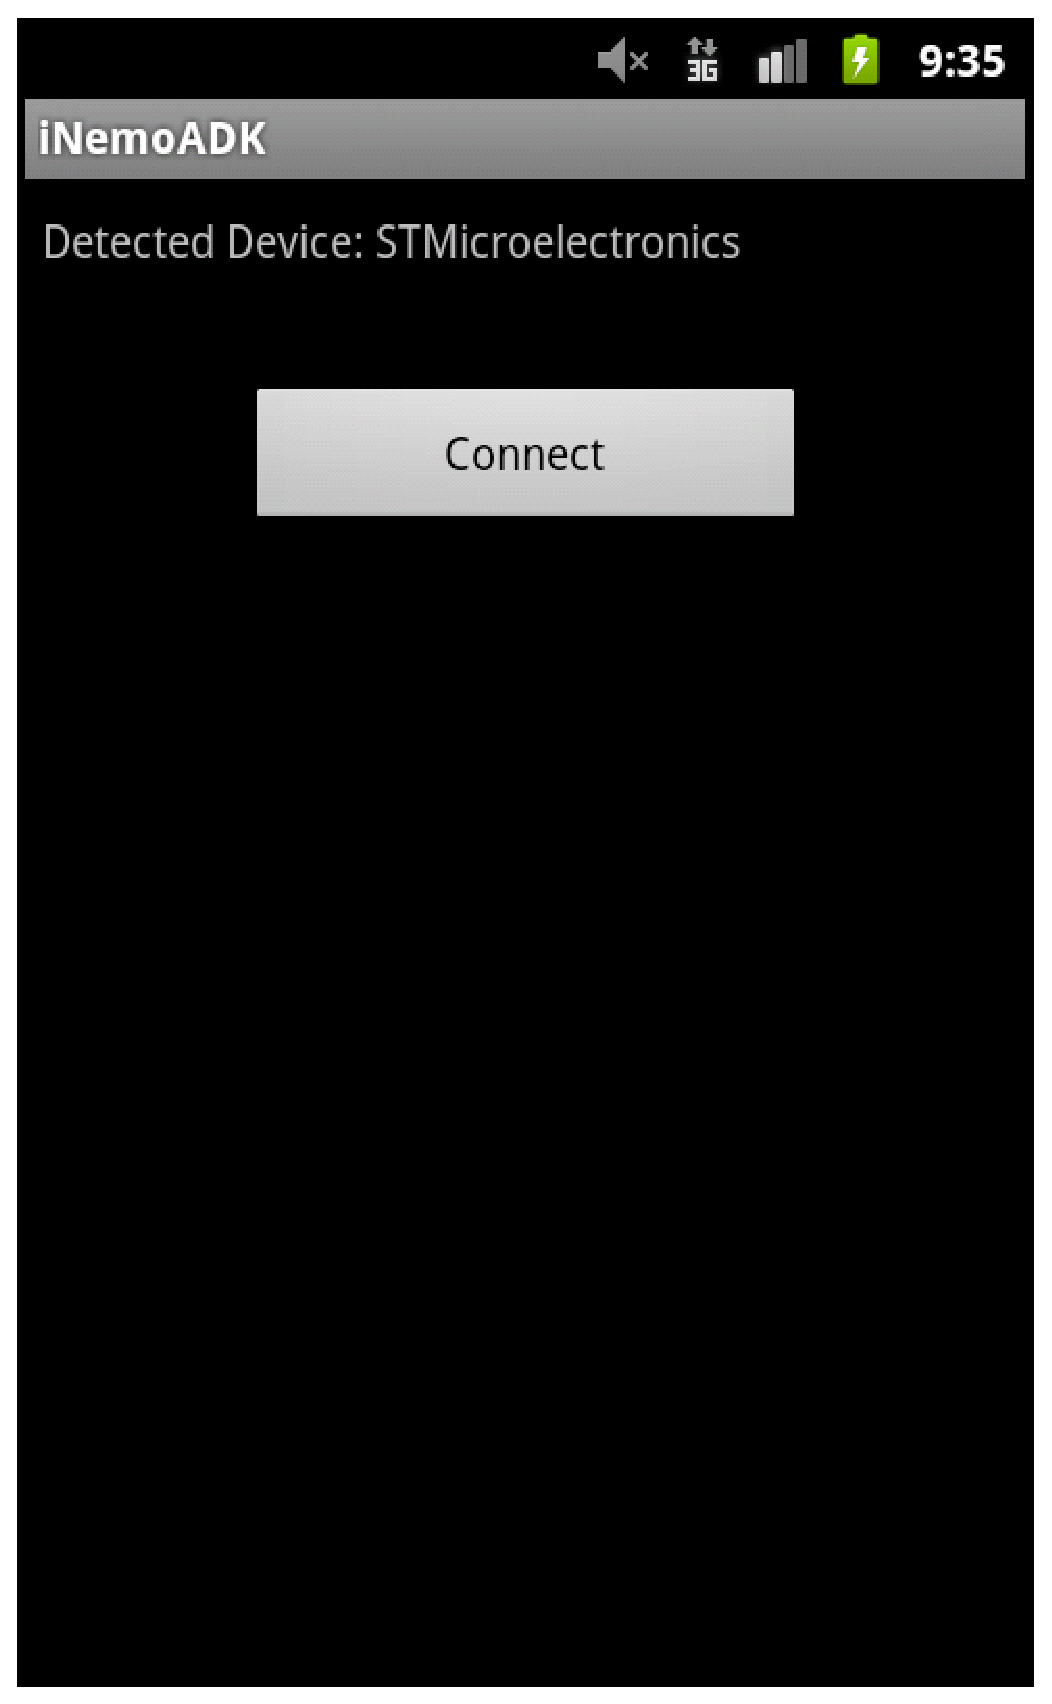
\includegraphics[width=0.6\linewidth]{pics/connect.eps}
	\captionof{figure}{Screen shown when the iNEMO board is attached.}
	\label{fig:connect}
\end{center}

When the connection is established, the application retrieves from the board information about the device identifier, the firmware and hardware version, the acquisition parameters and the sensors enabled. The user has the possibility to disconnect from the board, modify the acquisition parameters or start the acquisition (see {\bf Figure \ref{fig:connected}}).

\begin{center}
	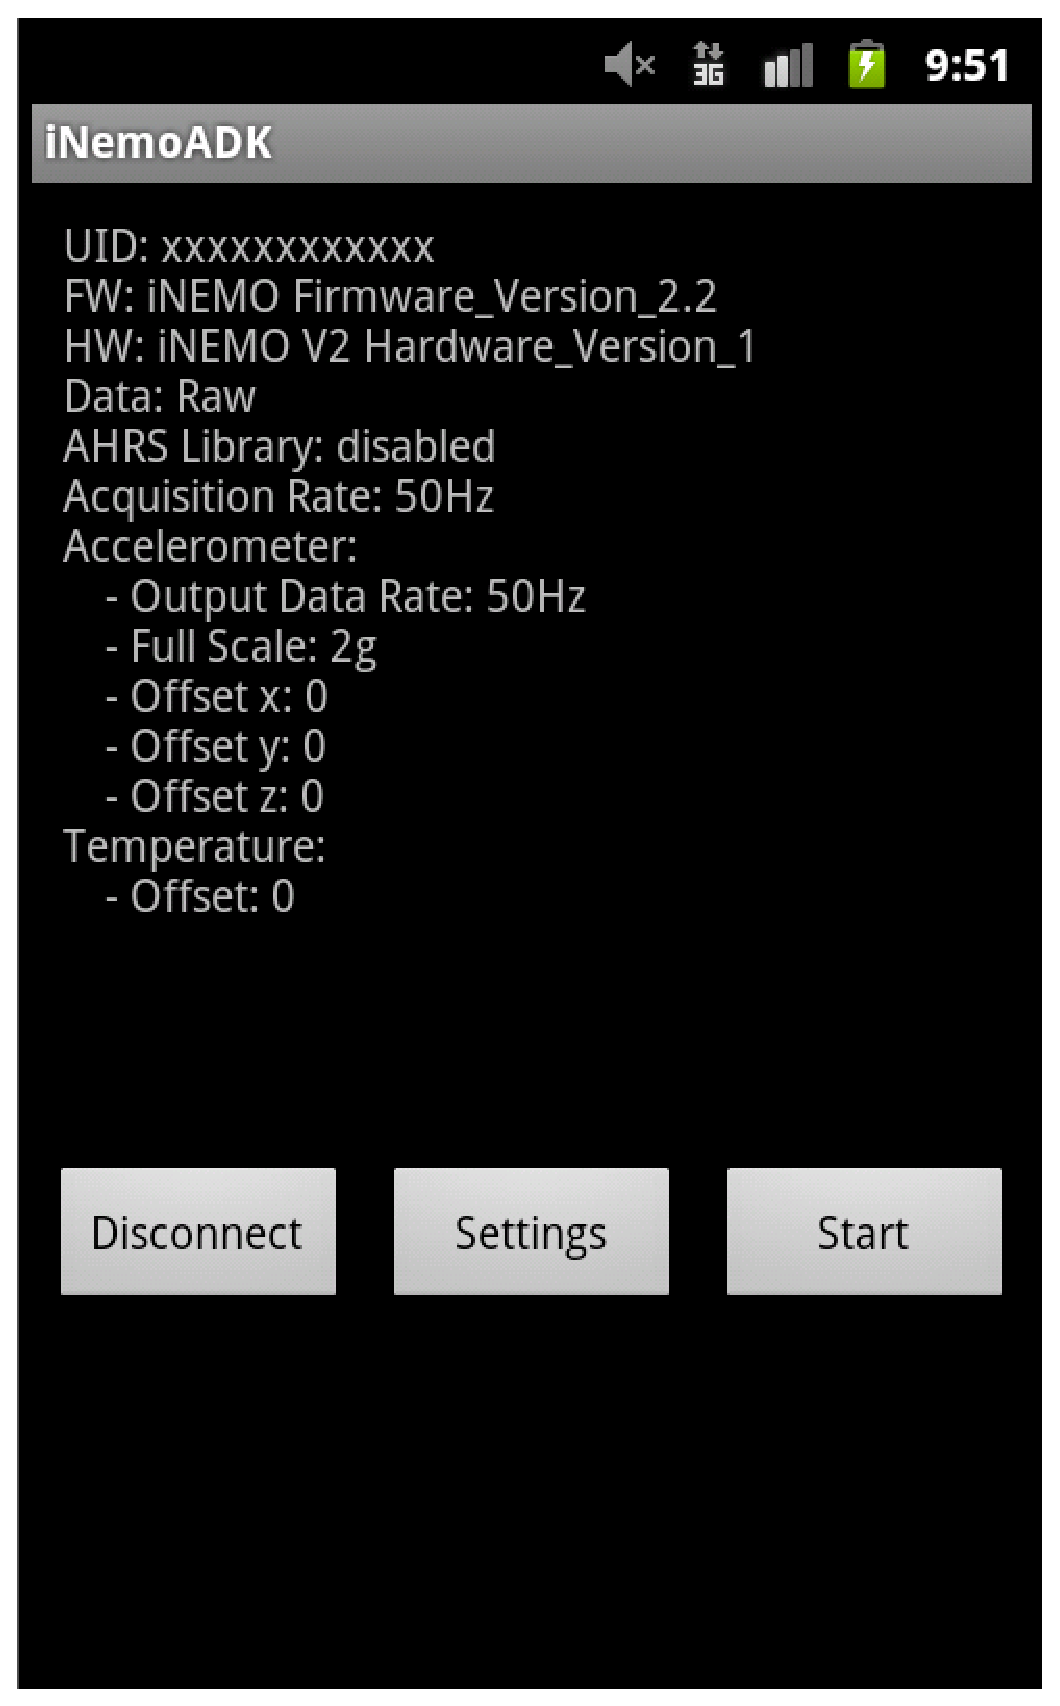
\includegraphics[width=0.6\linewidth]{pics/connected.eps}
	\captionof{figure}{Screen shown when the connection with the board is established.}
	\label{fig:connected}
\end{center}

The settings view ({\bf Figure \ref{fig:settings}}) allows the user to modify the acquisition parameters and to choose which sensors have to be enabled.

\begin{center}
	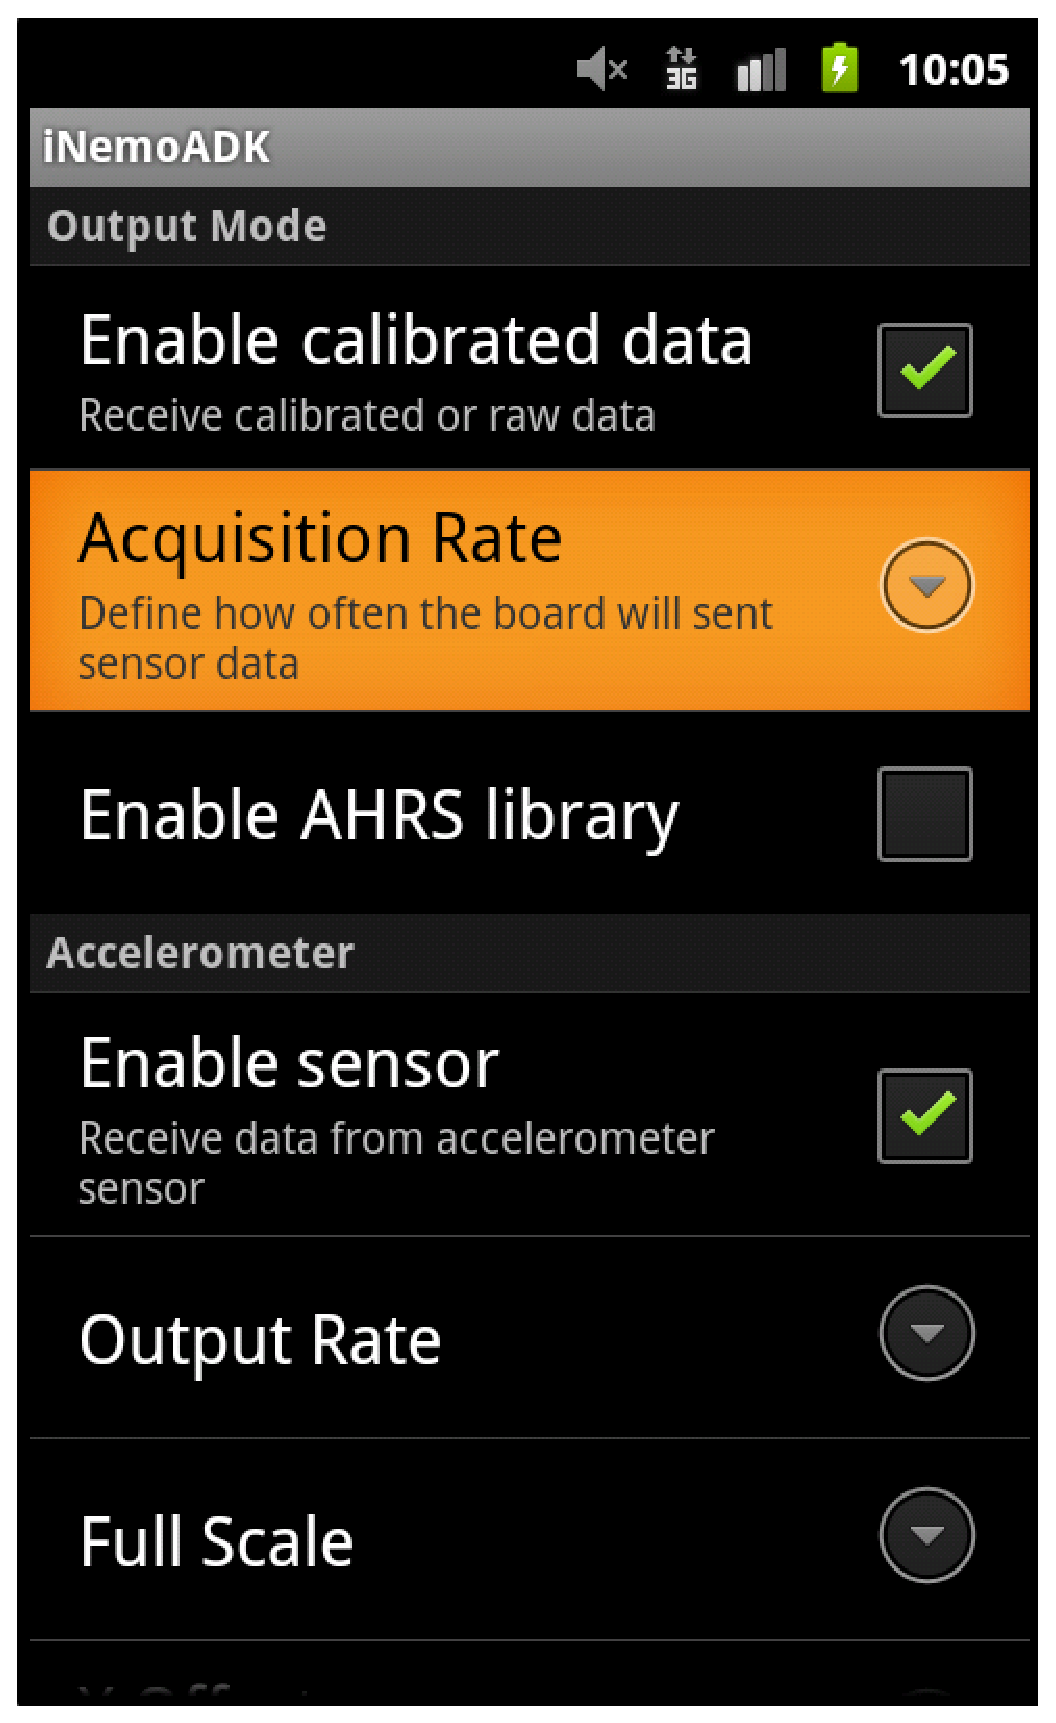
\includegraphics[width=0.6\linewidth]{pics/settings.eps}
	\captionof{figure}{Settings view.}
	\label{fig:settings}
\end{center}

Finally, during the acquisition phase, the application retrieves the data originated by the sensors of the board and shows them in a textual way (see {\bf Figure \ref{fig:acquisition}}). A future development is to shows sensor data in a graphical way (sliding graphs as in the Windows application iNEMO Suite).

\begin{center}
	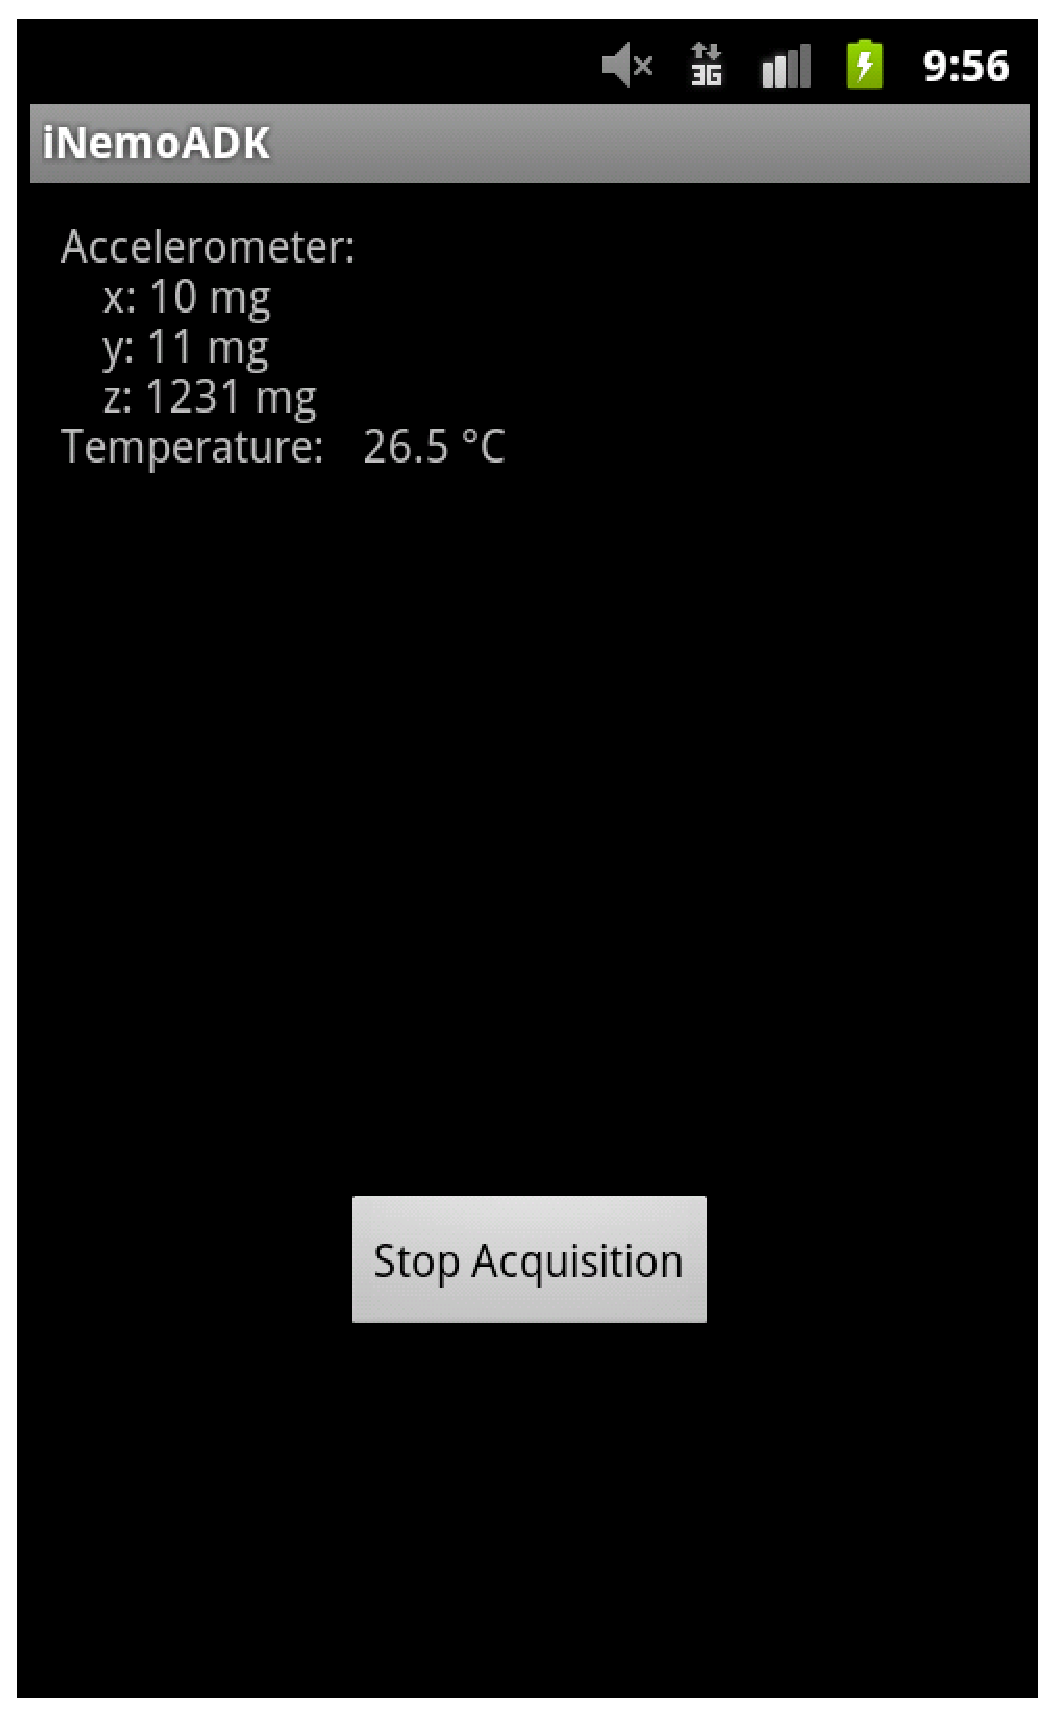
\includegraphics[width=0.6\linewidth]{pics/acquisition.eps}
	\captionof{figure}{Acquisition view.}
	\label{fig:acquisition}
\end{center}

As can be noticed, the layout is quite basic: another future development is to improve the graphic of the application.


